

In this section, we provide an overview of the second phase of
the construction of ASGs, illustrated in the middle of 
Figure \ref{fig:overview} by the rectangles labeled V.
We first describe the problems in building an ASG for the
{\CPP} language and then we describe the procedure we use
in Hylian to construct a language-complete ASG.


\begin{figure*}[htbp]
\centerline{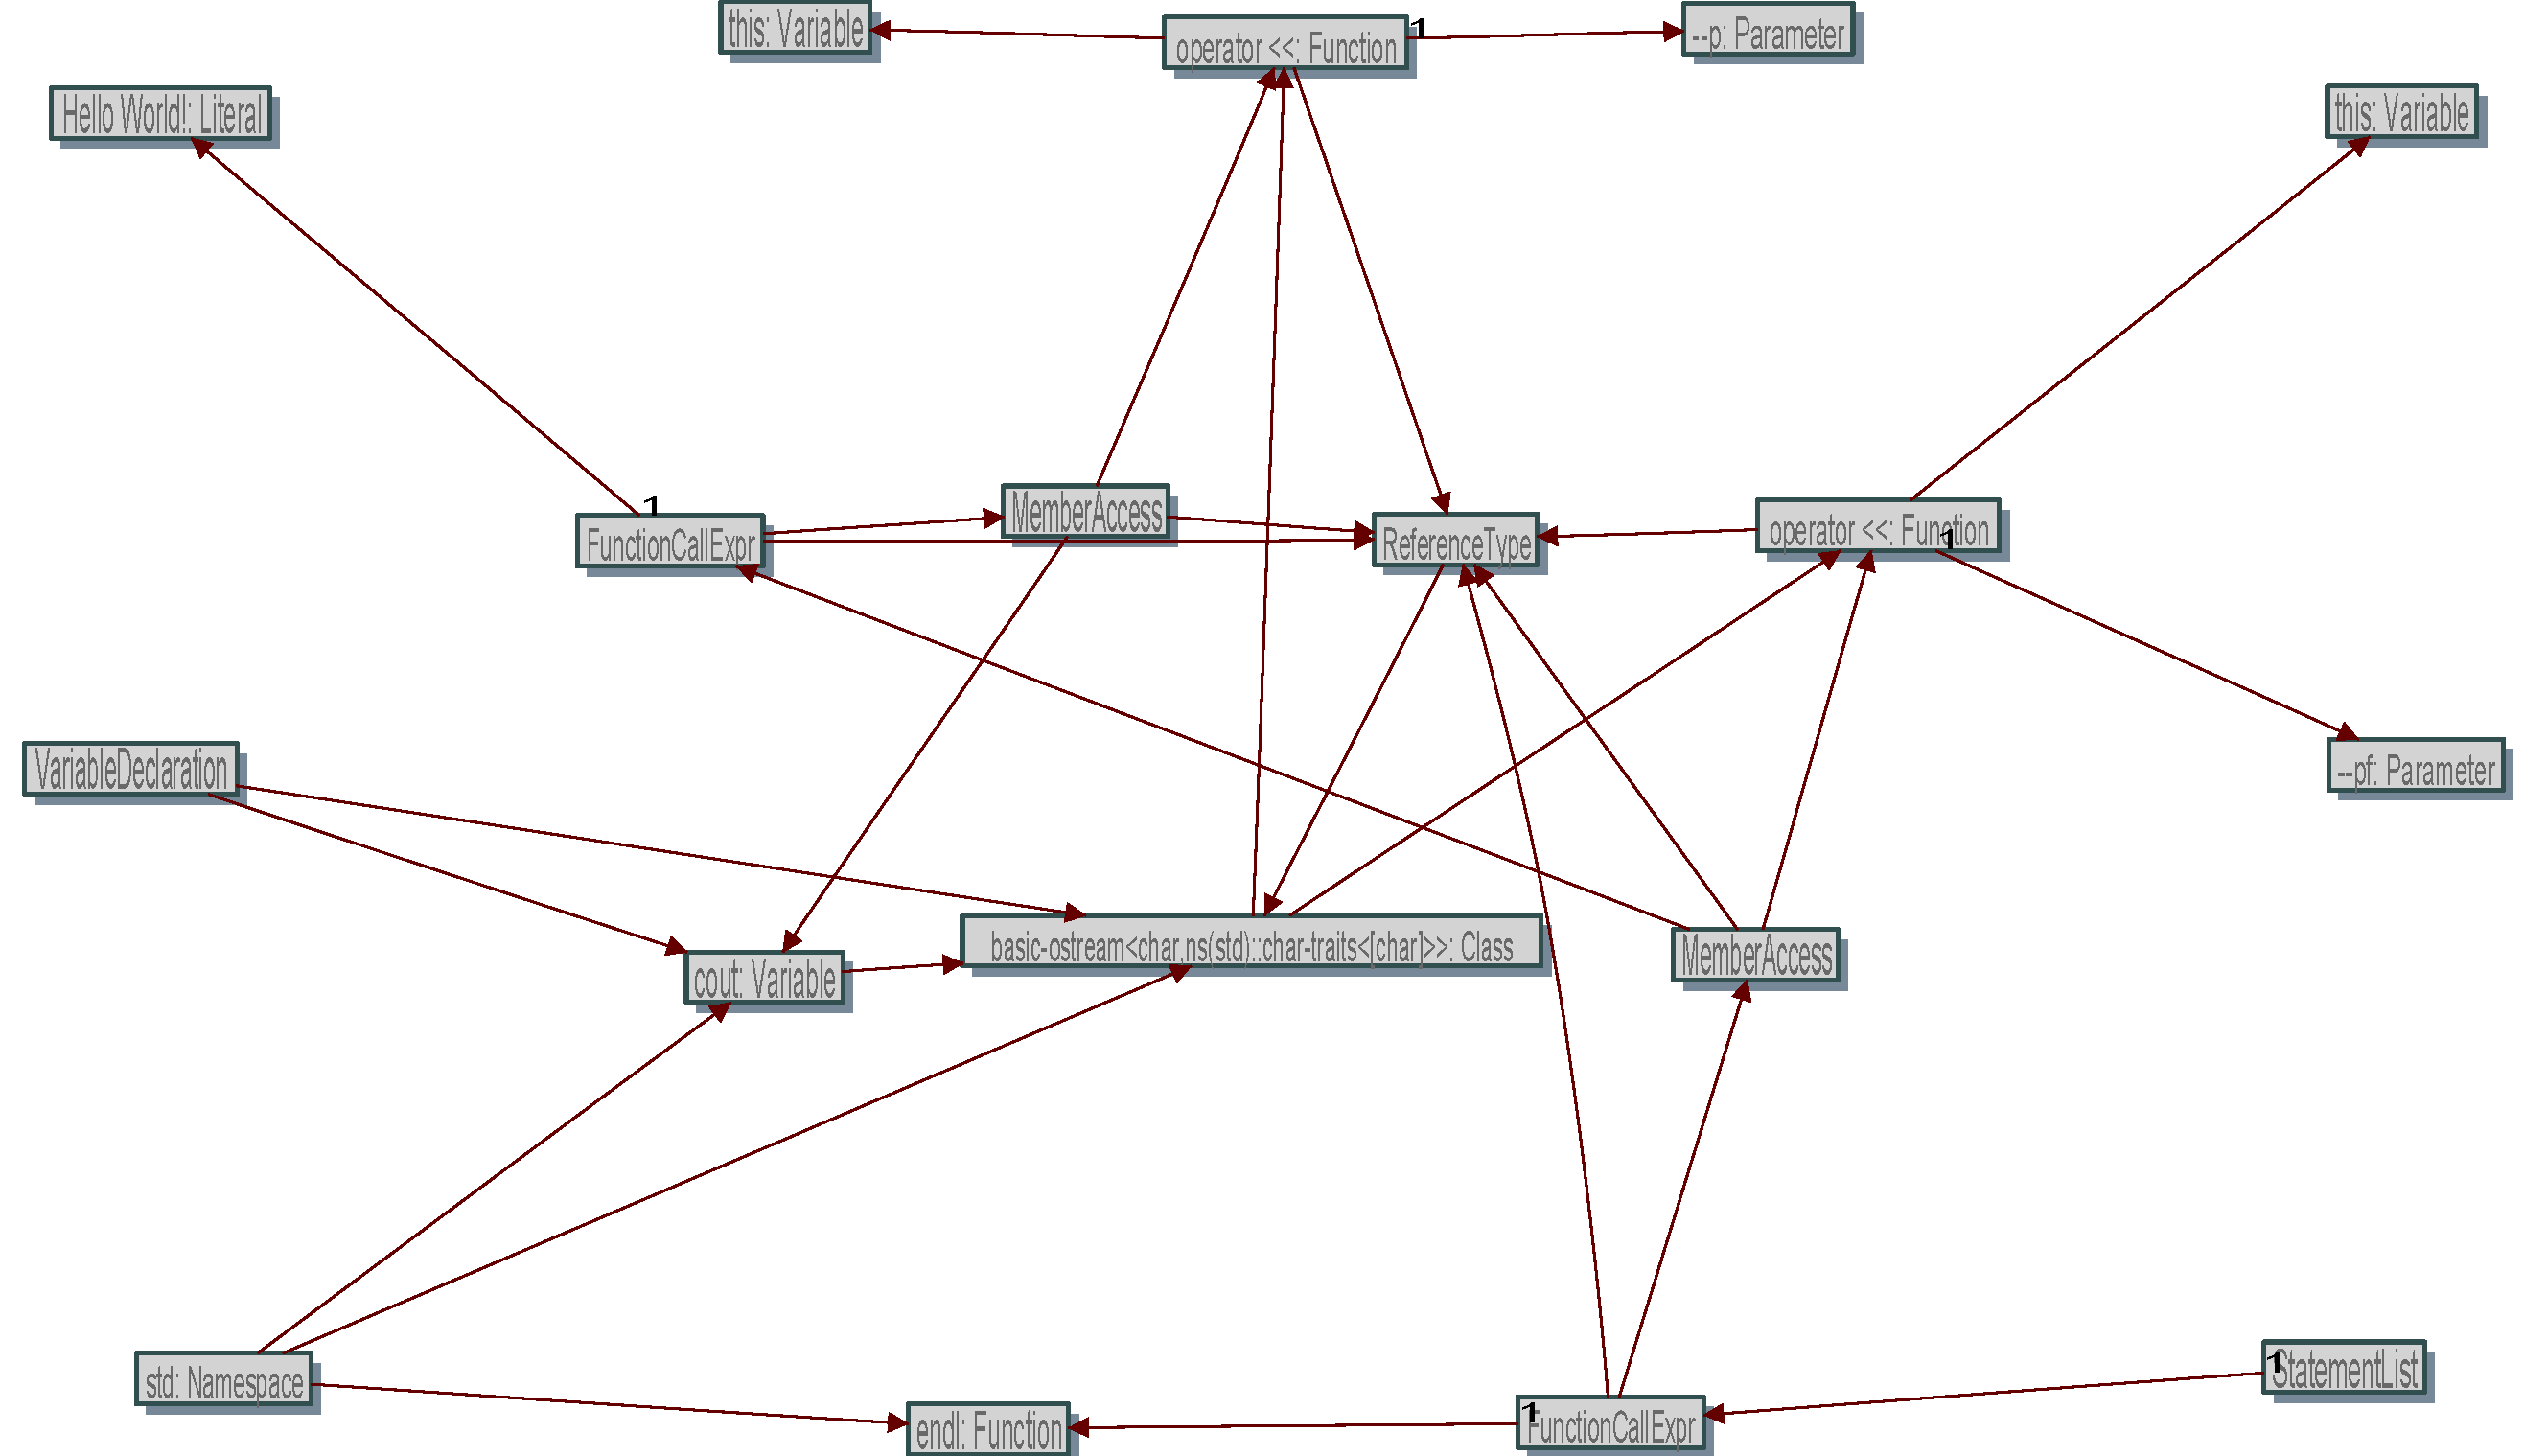
\includegraphics[scale=0.40]{figures/cpphello_full}}
\caption{A language-complete Abstract Semantic Graph for 
a \textsf{Hello World} program}
\label{fig:fullhello}
\figline
\end{figure*}


The attachment of type information to the names used in an
application is fairly straightforward if the program is written
in a procedural language such as C or Fortran. However, 
attaching semantic information to names used in applications
written in a multi-paradigm, composite 
language \cite{Stroustrup1994,dennythesis09}, 
such as {\CPP}, present unique challenges.
These features include data hiding, generics, multiple inheritance
and other constructs that make the attachment of semantic information
much more difficult than in the processing of procedural languages. 
These challenges comprise the bulk of the effort required for
the construction of the Hylian analysis system.

The most imposing of these challenges, name lookup, actually sounds 
uniquely trivial, yet a solution to this problem entails resolving
type information for virtually every production in the {\CPP} grammar.
Thus, name lookup is difficult firstly because of the breadth of
the problem, since the {\CPP} grammar is one of the largest grammars
in use, yet more importantly, is the most complex 
grammar \cite{Power-Malloy:04}.
For example, the {\sf impurity} metric applied to the {\CPP}
grammar shows that, at 85\%, the {\CPP} grammar contains a considerable
density in the edges in the closure of the call graph, especially
compared to the grammars for C, Java and C\#.
The {\sf impurity} metric, together with the application of McCabe's
metric to the {\CPP} grammar, provide further evidence of the
complexity, and the tight coupling of the {\CPP} grammar
productions \cite{Power-Malloy:04}.


As an illustrative example of the issues involved in name lookup
in {\CPP}, consider resolution of the simple three-operand expression 
for printing ``Hello World:''\\ 
\verb++\textsf{\textbf{int} main() \{ std::cout $\ll$ ``Hello, World!'' $\ll$ std::endl; \} }\\
The first operand is \textsf{std::cout} and its type is
{\sf std::ba\-sic\-\_ostream\-$<$char$>$}. The second operand,
a string literal, is type {\sf \textbf{const char}$\ast$}.
Resolving the correct implementation of \textsf{\textbf{operator}$\ll$}
involves examining seventeen methods of the instantiation of
\textsf{std::ba\-sic\_o\-stream}, and five function templates in the
\textsf{std} namespace, that accept a \textsf{std::basic\_ostream}
object as its first argument. 
The Hylian ASG construction algorithm compare the parameters 
for the partially-specialized function template in
\textsf{std::ba\-sic\_o\-stream} and find
those that most closely match the types 
of these first two operands.  When found, that function is instantiated,
inserted into the ASG, and the type of the subexpression is
\textsf{std::basic\_ostream}.
The full ASG for a {\sf hello world} program is illustrated 
in Figure \ref{fig:fullhello}.

\begin{figure}[ph]
   \centering
   \scriptsize
   \begin{tabular}{m{.03\textwidth}m{.7\textwidth}}
 ~1 & \verb++\textsf{\textbf{declare} \emph{tag}: XML tag} \\
 ~2 & \verb++\textsf{\textbf{declare} \emph{syntaxStack}: stack} \\
 ~3 & \verb++\textsf{\textbf{declare} \emph{semanticStack}: stack } \\
 ~4 & \verb++\textsf{\textbf{declare} \emph{parsetreeBuffer}: dictionary} \\
 ~5 & \verb++\textsf{\textbf{declare} \emph{currentParsetreeBuffer}: string} \\
 ~6 & \verb++\textsf{\textbf{declare} \emph{isBuffering}: boolean} \\
 ~7 & \verb++\textsf{\textbf{declare} \emph{currentTemplateDecl}: template declaration} \\
 ~8 & \\
 ~9 & \verb++\textsf{push an empty list onto \emph{semanticStack} and \emph{syntaxStack} } \\
 10 & \verb++\textsf{\emph{tag} $\leftarrow$ getTag()} \\
 11 & \verb++\textsf{\textbf{while} ( more tags in XML Parse Tree ) :} \\
 12 & \verb+  +\textsf{\textbf{if} (\emph{tag} \textbf{is} startTag) :} \\
 13 & \verb+    +\textsf{\textbf{if} ( \emph{tag} \textbf{is} template declaration \textbf{and not} \emph{isBuffering} ) :} \\
 14 & \verb+      +\textsf{\emph{currentParsetreeBuffer} $\leftarrow$ empty parse tree} \\
 15 & \verb+      +\textsf{\emph{currentTemplateDecl} $\leftarrow$ \emph{NULL}} \\
 16 & \verb+      +\textsf{\emph{isBuffering} $\leftarrow$ \emph{TRUE}} \\
 17 & \verb+    +\textsf{\textbf{if} ( \emph{isBuffering} ) :} \\
 18 & \verb+      +\textsf{\textbf{store} \emph{tag} \textbf{in} \emph{currentParsetreeBuffer}} \\
 19 & \verb+      +\textsf{\textbf{if} (\emph{currentTemplateDecl} \textbf{is not} \emph{NULL}) : } \\
 20 & \verb+        +\textsf{\textbf{continue} at top of while } \\
 21 & \verb+    +\textsf{\textbf{append} \emph{tag} to list at top of \emph{syntaxStack} } \\
 22 & \verb+    +\textsf{\textbf{if} ( \emph{tag} \textbf{is} tokenTag ) :} \\
 25 & \verb+      +\textsf{// keyword, constant, symbol, or identifier} \\
 26 & \verb+      +\textsf{\textbf{if} ( \emph{tag} is literal ) :} \\
 27 & \verb+        +\textsf{\textbf{determine} representation and type} \\
 28 & \verb+        +\textsf{\textbf{append} value of literal to list at top of \emph{semanticStack}} \\
 29 & \verb+      +\textsf{\textbf{else if} ( \emph{tag} \textbf{is} name ) :} \\
 30 & \verb+        +\textsf{\textbf{if} ( \emph{tag} \textbf{is} keyword ) :} \\
 31 & \verb+          +\textsf{\textbf{replace} `token' with actual keyword in list at top of} \\
 32 & \verb+             +\textsf{\emph{syntaxStack} (e.g., class)} \\
 33 & \verb+          +\textsf{\textbf{append} \emph{NULL} to list at top of \emph{semanticStack}} \\
 34 & \verb+        +\textsf{\textbf{else} :} \\
 35 & \verb+          +\textsf{\textbf{push} identifier onto list at top of \emph{semanticStack}} \\
 36 & \verb+      +\textsf{\textbf{else if} ( \emph{tag} is symbolTag ) :} \\
 37 & \verb+        +\textsf{\textbf{replace} `token' with symbol value (e.g., replace with `+')} \\
 38 & \verb+        +\textsf{\textbf{append} \emph{NULL} to list at top of \emph{semanticStack}} \\
 39 & \verb+    +\textsf{\textbf{else} :} \\
 40 & \verb+      +\textsf{\textbf{append} \emph{NULL} to list at top of \emph{semanticStack}} \\
 41 & \verb+  +\textsf{\textbf{else if} ( \emph{tag} \textbf{is} endTag ) :} \\
 42 & \verb+    +\textsf{\textbf{if} ( \emph{isBuffering} ) :} \\
 43 & \verb+      +\textsf{\textbf{store} \emph{tag} in \emph{currentParsetreeBuffer}} \\
 44 & \verb+    +\textsf{\textbf{if} (\textbf{not} \emph{isBuffering} \textbf{xor} \emph{currentTemplateDecl} \textbf{is not} \emph{NULL}) :} \\
 45 & \verb+      +\textsf{\textbf{call} function to perform semantic-action on\_tag\_name} \\
 46 & \verb+        +\textsf{i.e., for the tag "$<$/class\_head$>$" call on\_class\_head()} \\
 47 & \verb+      +\textsf{\textbf{pop} \emph{syntaxStack}} \\
 48 & \verb+      +\textsf{\textbf{pop} \emph{semanticStack}} \\
 49 & \verb+      +\textsf{\textbf{replace} \emph{NULL} in list at top of \emph{semanticStack} with result of} \\
 50 & \verb+        +\textsf{semantic-action, i.e. the semantic value of the production} \\
 51 & \\
 52 & \verb+    +\textsf{\textbf{if} (\emph{isBuffering} \textbf{and} \emph{currentTemplateDecl} \textbf{is not} \emph{NULL}) :} \\
 53 & \verb+      +\textsf{\textbf{add} to \emph{parsetreeBuffer}, where the key is the declaration, and the} \\
 54 & \verb+        +\textsf{value is the partially created buffer (in progress).} \\
 55 & \verb+    +\textsf{\textbf{if} (matching close of template\_declaration that started buffering) :} \\
 56  & \verb+       +\textsf{\emph{isBuffering} $\leftarrow$ \emph{FALSE}} \\
 57 & \verb+  +\textsf{\emph{tag} $\leftarrow$ getTag()} \\
   \end{tabular}
\caption{The algorithm used to convert a parse tree into a bottom-up style parse}
\label{fig:asgcons}
\shortline
\end{figure}

\subsection{Parsing parse trees expressed in XML}

The algorithm in Figure \ref{fig:asgcons} parses the XML representation of the parse-tree 
of the original user application code.  The parse-tree parser is a 
top-down SAX XML parser, but we prefer to handle the grammar productions
in bottom-up fashion. 
Thus, to simulate a bottom-up parse we must buffer the XML tags
that represent terminals and non-terminals from the original user
application code, and delay the semantic actions until a complete
sentence encountered.
The semantic action for each production is handled by a function
that accepts two lists: (1) a list of the syntax symbols, and (2)
a list of their corresponding semantic values.  The return value of
the semantic action function is the semantic value of that production.

To correctly handle template classes and functions, we delay total evaluation
of their subtree until we encounter a use later in the parse tree.
When a template definition is encountered, we must parse enough of its
tree to determine its declaration all the while buffering the entire subtree
for later use.  Once we determine the declaration, we stop handling semantic
actions until the matching close tag for the template declaration is reached.
We then store the template declaration and its corresponding parse tree
in a dictionary until a usage of the template requires instantiation.


%A summary of the actions required to build an ASG from an XML representation
%of a parse tree for a compilation unit is listed in Figure \ref{fig:asgcons}.
%The parse tree is result of the first phase of our system shown in 
%Figure \ref{fig:overview}.

\subsection{Overview of ASG construction}

To generate an ASG, we first prune 
the generated parse trees to eliminate unnecessary
non-terminals and empty productions. We then annotate the
pruned parse tree with semantic information, such as the type
or scope of a variable. In the case of templates, we must
build an ASG representation of the instantiated template.
After we have extended each of the parse trees with semantic
information to produce an ASG for each compilation unit,
we then {\em link}, or merge, the ASGs into a single
ASG for the entire program.
Exposition of the full algorithm for ASG construction is
beyond the scope of this paper. In this section,
we provide an overview of this construction  process.
The interested reader may consult reference \cite{duffythesis}
for details, and an algorithm, for ASG construction.


The algorithm for ASG construction uses seven data structures and a while
loop that examines each XML tag in turn. 
The first data structure, {\sf tag}, is the current XML tag.
The next two data structures facilitate a bottom up parse using
the tags from the top-down XML parser:
{\sf syntaxStack}, a stack of lists that contain terminals and
non-terminals encountered in the bottom-up parse;
and {\sf semanticStack}, a stack of lists that contain semantic values
encountered in the bottom up parse of the parse tree.
The final four data structures facilitate template declaration buffering
and instantiation:
{\sf parsetreeBuffer}, a dictionary that maps a template declaration
to its respective parse tree;
{\sf currentParsetreeBuffer}, a buffer for a parse tree of a template so
that when a template declaration is encountered the parse action is delayed 
until the template is instantiated and fully defined by its usage;
{\sf isBuffering}, a boolean indicating that the current tag
is the child of a template declaration;
and, finally,
{\sf currentTemplateDecl}, a handle for a declaration that
contains information to facilitate name lookup for the currently buffered
template declaration, which contains scope information, name, 
arguments for the template, and possibly information about parameters
to a function template.
